\documentclass[b5paper]{article}

\usepackage{tikz}

\begin{document}
%\begin{tikzpicture}[scale=1]
%    \pgfmathsetmacro{\e}{1.44022}   % eccentricity
%    \pgfmathsetmacro{\a}{1}
%    \pgfmathsetmacro{\b}{(\a*sqrt((\e)^2-1)} 
%    \draw plot[domain=-2:2] ({\a*cosh(\x)},{\b*sinh(\x)});
%    \draw plot[domain=-2:2] ({-\a*cosh(\x)},{\b*sinh(\x)});
%    \\
%\draw[scale=0.5,domain=-3.141:3.141,smooth,variable=\t] plot ({\t*sin(\t r)},{\t*cos(\t r)});
%%\draw plot[variable=\t,samples=1000,domain=-35:35] ({sec(\t)},{tan(\t)});
%\end{tikzpicture}

\centering
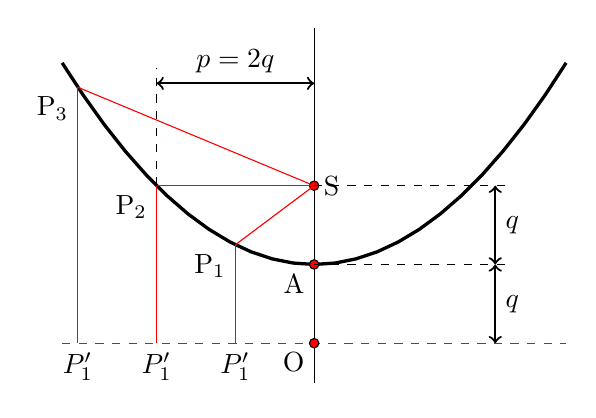
\begin{tikzpicture}
        \def\xmin{-3.2}
        \def\xmax{3.2}
        \def\ymin{-0.5}
        \def\ymax{4}

        \draw[dashed, red] (\xmin,0) -- (\xmax,0);% node[right] {$x$};
        \draw[black] (0,\ymin) -- (0,\ymax);% node[above] {$y$};

        \draw[color=black, very thick] plot [domain=\xmin:\xmax] (\x,{((\x)^2)/4 + 1)});
        \draw[fill=red] (0,2) circle(0.6mm) node[right] {S};
        \draw[fill=red] (0,1) circle(0.6mm) node[below left] {A};
        \draw[fill=red] (0,0) circle(0.6mm) node[below left] {O};
        
        \draw[red] (0,2) -- (-1, 1.25) node[below left, black] {P$_{1}$};
        \draw[red] (-1,0) node[below, black] {$P'_{1}$} -- (-1, 1.25);
        \draw[red] (0,2) -- (-2, 2) node[below left, black] {P$_{2}$};
        \draw[red] (-2,0) node[below, black] {$P'_{1}$} -- (-2, 2);
        \draw[red] (0,2) -- (-3, 3.25) node[below left, black] {P$_{3}$};
        \draw[red] (-3,0) node[below, black] {$P'_{1}$} -- (-3, 3.25);
        
        \draw[dashed, black] (-2,2) -- (-2,3.5);
        \draw[<->, black, thick] (0,3.3) -- (-2,3.3) node[midway, above, black] {$p=2q$};

		\draw[dashed, black] (0,1) -- (2.5,1);
		\draw[dashed, black] (0,2) -- (2.5,2);
		\draw[<->, black, thick] (2.3,0) -- (2.3,1) node[midway, right] {$q$};
		\draw[<->, black, thick] (2.3,1) -- (2.3,2) node[midway, right] {$q$};		
\end{tikzpicture}

\vspace{1cm}

\centering
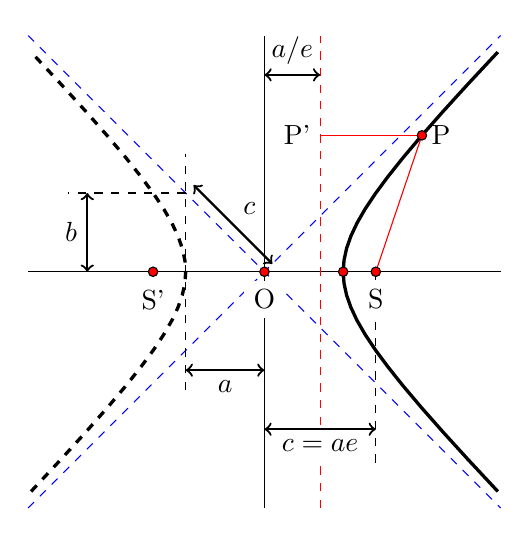
\begin{tikzpicture}
    \def\xmin{-3}
    \def\xmax{3}
    \def\ymin{-3}
    \def\ymax{3}

    \draw[black] (\xmin,0) -- (\xmax,0);% node[right] {$x$};
    \draw[black] (0,\ymin) -- (0,\ymax);% node[above] {$y$};
	
	\pgfmathsetmacro{\e}{1.41421356237}   % eccentricity
    \pgfmathsetmacro{\a}{1}
    \pgfmathsetmacro{\b}{(\a*sqrt((\e)^2-1)} 
    \draw[very thick] plot[domain=-1.75:1.75] ({\a*cosh(\x)},{\b*sinh(\x)});
    \draw[dashed, very thick] plot[domain=-1.75:1.75] ({-\a*cosh(\x)},{\b*sinh(\x)});
    
    \draw[dashed, blue] plot[domain=-3:3] (\x,\x);
    \draw[dashed, blue] plot[domain=-3:3] (\x,-\x);
    
	\draw[dashed, black] (-1,-1.5) -- (-1,1.5);
	\draw[<->, black, thick] (0,-1.25) -- (-1,-1.25) node[midway, below, black] {$a$};
	\draw[dashed, black] (-1,1) -- (-2.5,1);
	\draw[<->, black, thick] (-2.25,0) -- (-2.25,1) node[midway, left, black] {$b$};
	\draw[<->, black, thick] (0.1,0.1) -- (-0.9,1.1) node[midway, above right, black] {$c$};
	\draw[dashed, black] (1.41421356237,0) -- (1.41421356237,-2.5);
	\draw[dashed, red] (0.70710678119,-3) -- (0.70710678119,3);	
	\draw[<->, black, thick] (0,-2) -- (1.41421356237,-2) node[midway, below, black, fill=white] {$c=ae$};
	\draw[<->, black, thick] (0,2.5) -- (0.70710678119,2.5) node[midway, above, black] {$a/e$};
	\draw[red] (1.41421356237,0) -- (2,1.732050808);
	\draw[red] (0.70710678119,1.732050808) node[left,black] {P'} -- (2,1.732050808);
	
	\draw[fill=red] (1.41421356237,0) circle(0.6mm) node[below=3, fill=white] {S}; 
	\draw[fill=red] (-1.41421356237,0) circle(0.6mm) node[below=3] {S'};     
	\draw[fill=red] (0,0) circle(0.6mm) node[below=3, fill=white] {O};
	\draw[fill=red] (1,0) circle(0.6mm); %node[below left=0.5] {A}; 
	\draw[fill=red] (2,1.732050808) circle(0.6mm) node[right] {P};   
\end{tikzpicture}

\end{document}